\documentclass[conference]{IEEEtran}
\IEEEoverridecommandlockouts

% Packages
\usepackage{cite}
\usepackage{amsmath,amsfonts}
\usepackage{algorithm}
\usepackage{algpseudocode}
\usepackage{graphicx}
\usepackage{textcomp}
\usepackage{xcolor}
\usepackage{booktabs}
\usepackage{adjustbox}
\usepackage{listings}

\usepackage{verbatim}
\usepackage{multirow}

\usepackage{subcaption}

%\def\BibTeX{{\rm B\kern-.05em{\sc i\kern-.025em b}\kern-.08em
    %T\kern-.1667em\lower.7ex\hbox{E}\kern-.125emX}}

\begin{document}

\author{}
\title{Deliverable report \\
\footnotesize \textit{"Diego Oniarti": Mat: 257835, \texttt{diego.oniarti@studenti.unitn.it}, GitRepo: \texttt{https://github.com/diego-oniarti/GPU-Computing-2025-257835}}}

\maketitle

\begin{abstract}
% [max 200 words]\\
% The sparse matrix-dense vector multiplication (SpMV) is a common linear algebra operation involving a sparse matrix and a dense vector. SpMV is widely used in many real-world applications such as \dots
% 
% This deliverable discusses \dots
Sparse matrix-dense vector multiplication (SpMV) is an operation consisting of the multiplication between a sparse matrix and a dense vector. It can be seen as a specific case of the general dot product between two matrices, where one mostly contains zeros and the other has a row size of 1.

This deliverable discusses some of the ways these constraints on the matrices involved in the multiplication can be leveraged to improve the performance of the operation.\\
The techniques used will revolve around efficient cache usage and parallelization through the use of GPUs.
\end{abstract}

\begin{IEEEkeywords}
Sparse Matrix, SpMV, CUDA, Parallelization, Storage Format
\end{IEEEkeywords}

\section{Introduction}
% [max 300 words]\\
% Introduce SpMV application and its parallelization challenges \dots
SpMV is an operation that is used in many different fields like graph algorithms, graphics processing, numerical analysis, and conjugate gradients\cite{ZHUO2011709}. Sparse matrices appear naturally in many fields of computer science and data analysis, and the multiplication of these matrices by some vector can have different purposes and effects.

\section{Problem Statement}
% Define the problem statement, including a description of the storage format used and a brief discussion of the parallelization approach (e.g., using CUDA).
% \subsection{Storage Format}
% Details about the format (e.g., CSR, COO, etc.) \dots
% 
% \subsection{Parallelization}
% Describe the CUDA implementation approach \dots
Sparse matrix-dense vector multiplication poses many difficulties, mainly relating to the usage of memory, cache, and the efficiency of the parallelization approach.

\subsection{Storage Format}
The way the matrix is stored into memory can highly effect the performance of any algorithm iterating through its elements. Different strategies exist, each having pros and cons, and this deliverable will detail implementations that involve the Compressed Sparse Row (CSR) format.

This format represents the matrix through the use of three vectors:
\begin{enumerate}
    \item \textbf{Values} containing all and only the nonzero values contained in the matrix. The values appear in the vector in the same order as they appear in the matrix if scanned top to bottom and left to right.
    \item \textbf{Xs} containing the $x$ indices of the nonzero elements. The elements in this vector are sorted in the same way as in the values vector, and the two can be aligned.
    \item \textbf{Ys} has one element per row plus one. It contains the prefix sum of the count of nonzero values for each line.
\end{enumerate}
This matrix representation saves space by not explicitly storing the nil entries of the matrix. The additional information (Xs and Ys) is negligible with respect to the size of the matrix if the values are sparse enough.

Furthermore, by storing the values in a sorted order, we can take advantage of spatial locality while iterating over the matrix.

\subsection{Parallelization}
The first approach presented will focus on the row-wise parallelization of the multiplication. This choice was made because the result in each cell of the result matrix is independent from every other cell, so there won't be any conflict or synchronization issue when computing them in parallel.\\
Each thread will independently iterate through it's assigned row of the matrix, multiply the elements by the corresponding ones in the vector, sum them, and store the result.

A further improvement on this technique will further parallelize the multiplication along each row by allocating multiple threads to it.

\subsection{Cache Usage}
This deliverable already showed how spatial locality is well taken advantage of during the scan of the matrix. The access to the vector, however, is mostly random, making cache hits more rare.\\
One of the implementations that will be shown sacrifices some of the spatial locality of the matrix to gain temporal locality on the vector. By dividing the multiplication procedure into smaller chunks, we can theoretically get better cache usage in the case highly structured matrices.

% \section{State of the Art}
% Describe the available library solutions for the SpMV problem, including references and citations.

\section{Methodology and Contributions}\label{sec:methodology}

% Describe the methodology used during the analysis, the compared algorithms and the expected outcomes. Use pseudo-codes like Algorithm \ref{alg:COOaggr} to describe your own implemented kernels.
% 
% \noindent Include at least the following implementations:
% \begin{itemize}
%     \item Naive CPU implementation
%     \item Optimised CPU implementation based on cache behaviour
%     \item GPU naive implementation
% \end{itemize}
% 
% \noindent For the analysis include
% \begin{itemize}
%     \item Valgrind and runtime comparison between the CPU implementations 
%     \item Runtime CPU vs GPU comparison looping over different matrix dimensions
% \end{itemize}
% 
% \begin{algorithm}[ht!]
% \caption{Algorithm for the vector addition}
% \algorithmicrequire~The input vectors $a$ and $b$ of size $nnz$.
% \begin{algorithmic}[1]
% \Procedure{Function}{$a$, $b$, $nnz$}
% \State $c \gets \emptyset$
% \For{$i$ in $\{1 \dots nnz\}$ \textbf{parallel}}
% \State $c[i] = a[i] + b[i]$
% \EndFor
% \State \textbf{return} $c$\Comment{the result vector}
% \EndProcedure
% \end{algorithmic}
% \label{alg:COOaggr}
% \end{algorithm}

In this section I'm gonna illustrate four different implementations for the multiplication. The first one is a straightforward multiplication on the CPU, made faster by the CSR representation of the matrix. The second one tries to take better advantage of the cache by accessing the data in a different pattern. The third one works like the first, but the computation for each line is done simultaneously on the GPU. Finally, the fourth one is a further improvement on the third. In this implementation, instead of each row being assigned a single thread, it will get 32.

\subsection{Naive CPU}
This is the simplest approach which iterates through the nonzero values, uses the \textit{x} index to indirectly access the vector, and accumulates the result for each line.
\begin{algorithm}[ht!]
    \caption{Naive implementation on the CPU}
    \algorithmicrequire~The input vectors $vals$ and $xs$ of size $nnz$, the vector $ys$ of size $ncols$, and the vector $vec$ to multiply the matrix with.
    \begin{algorithmic}[1]
        \Procedure{Multiply}{$vals$, $xs$, $ys$, $vec$, $nnz$, $nrows$}
        \State $result \gets array[nrows]$
        \For{$i$ in $[0 \dots nrows)$} % \Comment{Iterate through the rows}
        \State $result[i] \gets 0$
        \For{$j$ in $[ys[i]\dots ys[i+1])$} % \Comment{Iterate through the elements in the row}
            \State $result[i]$ += $vals[j] * vec[xs[j]]$
            \EndFor
        \EndFor
        \State \textbf{return} $result$ %\Comment{the result vector}
        \EndProcedure
    \end{algorithmic}
    \label{algo:CPU}
\end{algorithm}

\subsection{CPU - chunked}
This implementation attempts to increase temporal-locality when accessing the vector, sacrificing some of the spatial-locality in the access to the matrix. The algorithm iterates through the vector in chunks, it then iterates through the rows and computes the product between the chunk of vector and the corresponding chunk in the line, adding the partial sum to the total for said row.\\
This approach requires the storage of the current index for each row and introduces the chunk size as an hyperparameter ($8$ should be a good value, ensuring the whole chuck of the vector remains cached).
\begin{algorithm}[ht!]
    \caption{Chunked CPU implementation}
    \begin{algorithmic}[1]
        \Procedure{Multiply}{$vals$, $xs$, $ys$, $vec$, $nnz$, $nrows$, $ncols$}
        \State $result \gets array[nrows]$
        \State $rc \gets array[nrows]$\Comment{Row Counters}
        \For{$i$ in $[0\dots nrows)$}
        \State $rc \gets ys[i]$ \Comment{Counters start at the beginning of the row}
        \EndFor
        \For{$i$ in $[0\dots nrows)$}
        \State $result[i]\gets 0$
        \EndFor

        \For {$i=0$; $i<ncols$; $i+=span$}
        \For {$r$ in $[0\dots nrows)$}
        \State $line\_end \gets ys[r+1]$
        \While {$rc[r] < line\_end$ and $i\leq xs[rc[r]] < i+span$}
        \State $result[r] += vals[rc[r]] * vec[xs[rc[r]]]$
        \State $rc[r]++$
        \EndWhile
        \EndFor
        \EndFor
        \State\Return result
        \EndProcedure
    \end{algorithmic}
    \label{algo:chunks}
\end{algorithm}

\subsection{Naive GPU}
The GPU implementation uses CUDA to parallelize the product along the rows. The algorithm works exactly as \textbf{Algorithm \ref{algo:CPU}}, with the difference that its ran on $nrows$ threads, and each thread only performs the inner loop.

The parameters are the same, with the exception of the additional return vector. While the CPU implementation allocated the vector inside the function, the GPU kernel receives a global array where to store the results.
\begin{algorithm}[ht!]
    \caption{Naive implementation on the GPU}
    \begin{algorithmic}[1]
        \Procedure{Kernel}{$vals$, $xs$, $ys$, $vec$, $nnz$, $nrows$, $result$}
        \State $i \gets thread\_id + block\_id\cdot block\_size$
        \If {$i>=nrows$}\Comment{Early return}
        \State \textbf{return}
        \EndIf
        \State $result[i] \gets 0$
        \For{$j$ in $[ys[i]\dots ys[i+1])$} % \Comment{Iterate through the elements in the row}
        \State $result[i]$ += $vals[j] * vec[xs[j]]$
        \EndFor
        \EndProcedure
    \end{algorithmic}
    \label{algo:GPU}
\end{algorithm}

\subsection{Improved GPU}
An improvement on the first GPU implementation consists in allocating one warp per row instead of a single thread. The threads in the warp iterate over the row with a stride equal to the warp size and store their partial sum in a buffer. A reduction is then performed to sum together the partial sums, and the thread with the lowest id finally moves the result into the result vector.

The buffer is a vector stored in global memory. A further improvement would be moving it to shared memory, but it is out of the scope of this deliverable.

\section{System Description and Experimental Set-up}
% Use this section to describe system, dataset and experimental set-up.
Each run has been performed with $3$ warm-up cycles and $10$ timed runs, which are then averaged. The timing of the CPU implementation was measured with the \texttt{gettimeofday} function from the standard library, while the GPU kernels were timed using CUDA events.

Additionally, the GPU kernels have been tested with different block sizes, ranging from 32 to 1024 and doubling each time.

\subsection{System Description}
% Describe the used system and the software environment (CUDA version, GCC version, \dots). Decide which information are valuable to group into a table like Table \ref{tab:system_description} and which are more valuable to be described in the text.

All the code has been ran on the Baldo cluster, with an AMD EPYC 9334 32-CORE Processor and a NVIDIA A30 GPU.\\
The CUDA version being used is 12.5.0 and the code has been compiled with NVCC 12.5.
The theoretical memory bandwidth for the GPU is around $933$GB/s.

\subsection{Dataset description}
Each of the algorithms was ran on 4 different kind of matrices, with different sizes, types of data, and levels of organization.\\
Three of the matrices have been taken from SuiteSparse Matrix Collection, while one is generated at runtime with a completely random distribution.
\begin{table}[ht!]
    \centering
    \begin{adjustbox}{width=\columnwidth}
        \begin{tabular}{l|r|r|rl|l}
            name & rows & columns & nonzeros & (\%) & type \\
            \hline
            lp\_ganges\footnote & 1309 & 1706 & 6937 & 0.3106\% & real \\
            delaunay\_n23\footnotemark & 8388608 & 8388608 & 50331568 & 7.152546e-5\% & binary \\
            Stanford\_Berkeley\footnotemark & 683446 & 683446 & 7583376 & 0.001624\% & binary \\
            random & 30000 & 20000 & 6001585 & 1.000264\% & real \\
        \end{tabular}
    \end{adjustbox}
    \caption{Test matrices}
    \label{tab:matrices}
\end{table}
\footnotetext[1]{https://www.cise.ufl.edu/research/sparse/matrices/LPnetlib/lp\_ganges}
\footnotetext[2]{https://www.cise.ufl.edu/research/sparse/matrices/DIMACS10/delaunay\_n23}
\footnotetext[3]{https://www.cise.ufl.edu/research/sparse/matrices/Kamvar/Stanford\_Berkeley}

\begin{figure}
    \centering
    \begin{subfigure}[b]{0.45\linewidth}
        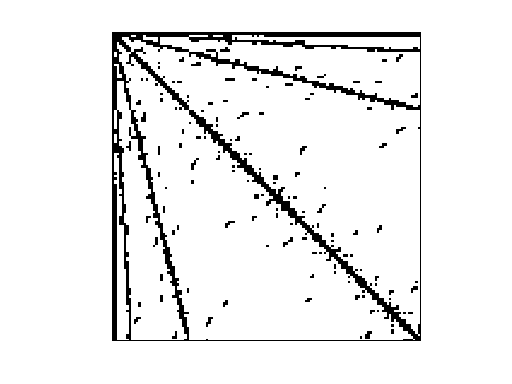
\includegraphics[width=\linewidth]{images/delaunay_n23.png}
        \caption{Delaunay Graph}
        \label{fig:delaunay_n23}
    \end{subfigure}
    \hfill
    \begin{subfigure}[b]{0.45\linewidth}
        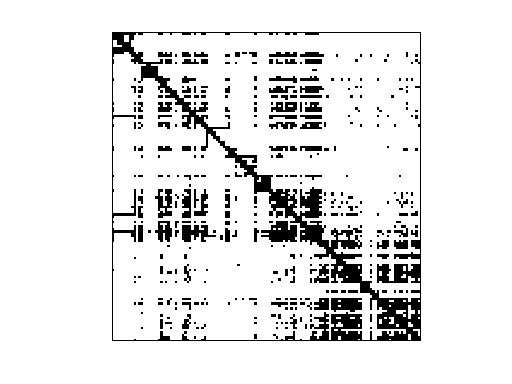
\includegraphics[width=\linewidth]{images/Stanford_Berkeley.png}
        \caption{Stanford-Berkeley Dataset}
        \label{fig:stanford_berkeley}
    \end{subfigure}
    \vspace{0.5cm}
    \begin{subfigure}[b]{0.45\linewidth}
        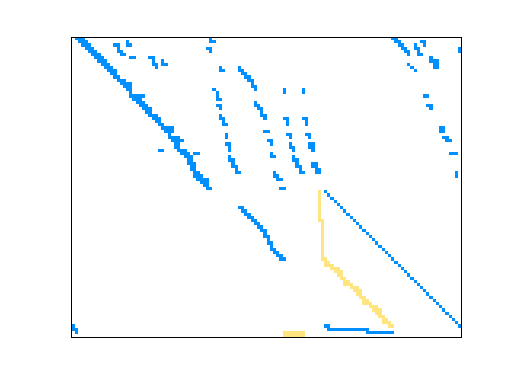
\includegraphics[width=\linewidth]{images/lp_ganges.png}
        \caption{LP-Ganges Dataset}
        \label{fig:lp_ganges}
    \end{subfigure}
    
    \caption{Datasets distributions}
    \label{fig:Dataset-images}
\end{figure}

\section{Experimental Results}
% Present and discuss results. Include plots and tables when required (like Figure \ref{fig:enter-label}). Do not simply describe the figures; criticise the achieved results by underlining how they confirm/differ from the expected outcomes described in Section \ref{sec:methodology}.
% 
% \begin{figure}
%     \centering
%     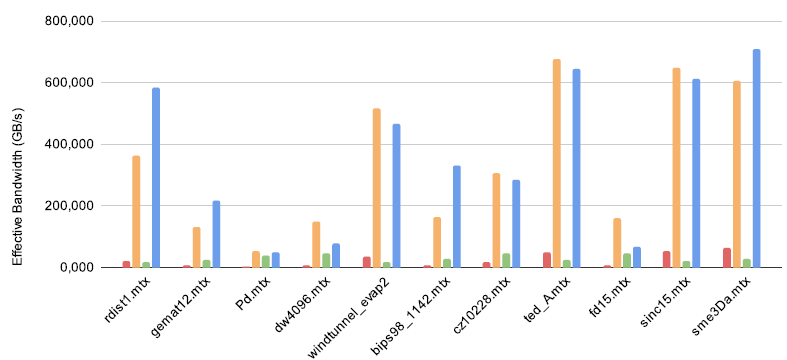
\includegraphics[width=0.95\linewidth]{SampleImage.png}
%     \caption{Caption}
%     \label{fig:enter-label}
% \end{figure}

The results immediately show that my assumptions on the chunked CPU implementation were wrong. Each run of that algorithm take up to double the time of the naive implementation on small matrices, and goes past the 5 minutes of allotted time on larger matrices.\\
The implementation aimed at taking advantage of temporal locality when reading the vector, sacrificing some of the spatial locality when reading the matrix. This trade-off, combined with the added complexity in iterating over the rows multiple times and handling the \textit{row\_counters} vector, has proven not to be worth it.

\begin{table}[ht!]
    \centering
    \begin{adjustbox}{width=\columnwidth}
        \begin{tabular}{l|ccc|ccc|ccc|ccc}
            \toprule
& \multicolumn{3}{c}{Delaunay} & \multicolumn{3}{c}{LP\_Ganges} & \multicolumn{3}{c}{stanford} & \multicolumn{3}{c}{random} \\
\cmidrule(lr){2-4} \cmidrule(lr){5-7} \cmidrule(lr){8-10} \cmidrule(lr){11-13}
& CPU & thread & warp & CPU & thread & warp & CPU & thread & warp & CPU & thread & warp \\
\midrule
            threads per block & - & 256 & 128 & - & 1024 & 128 & - & 64 & 128 & - & 1024 & 64 \\
            mean time (ms) & 185.34 & 0.466 & 8.013 & 26.7 & 0.016 & 0.012 & 29 & 5.202 & 0.959 & 19.586 & 0.447 & 0.104 \\
            deviation (ms) & 2.288 & 0.001 & 0.003 & 1.567 & 0 & 0.001 & 0.065 & 0.249 & 0.017 & 0.017 & 0.001 & 0.001 \\
            bandwidth (GB/s) & 1.629 & 647.73 & 37.69 & 0.004 & 6.873 & 9.646 & 2.342 & 13.239 & 71.791 & 2.464 & 108 & 462.88 \\
            FLOPS & 271560 & 107955022 & 6280994 & 519 & 846801 & 1188493 & 515870 & 2915663 & 15810505 & 612323 & 26843502 & 115047352 \\
            \bottomrule
        \end{tabular}
    \end{adjustbox}
    \caption{Experimental results}
    \label{tab:results}
\end{table}
\textbf{Table \ref{tab:results}} shows the results of the three working algorithms on each dataset. The GPU implementations have been tested with different block sizes, but only the ones with the best results are shown.

The bandwidth of each algorithm, as shown in \textbf{Figure \ref{fig:chart}}, mostly follows a clear trend, with the increasing amount of parallelization leading to better performances. 

The only outlier in this trend is the Delaunay dataset, with the reason most likely being the first row of the graph. Looking at the distribution of the values in \textbf{Figure \ref{fig:delaunay_n23}}, it is visible that the first row of the graph is dense. This fact can possibly bring the second algorithm to take better advantage of the cache, beating the advantage that the third one would have had.

\begin{figure}
    \centering
    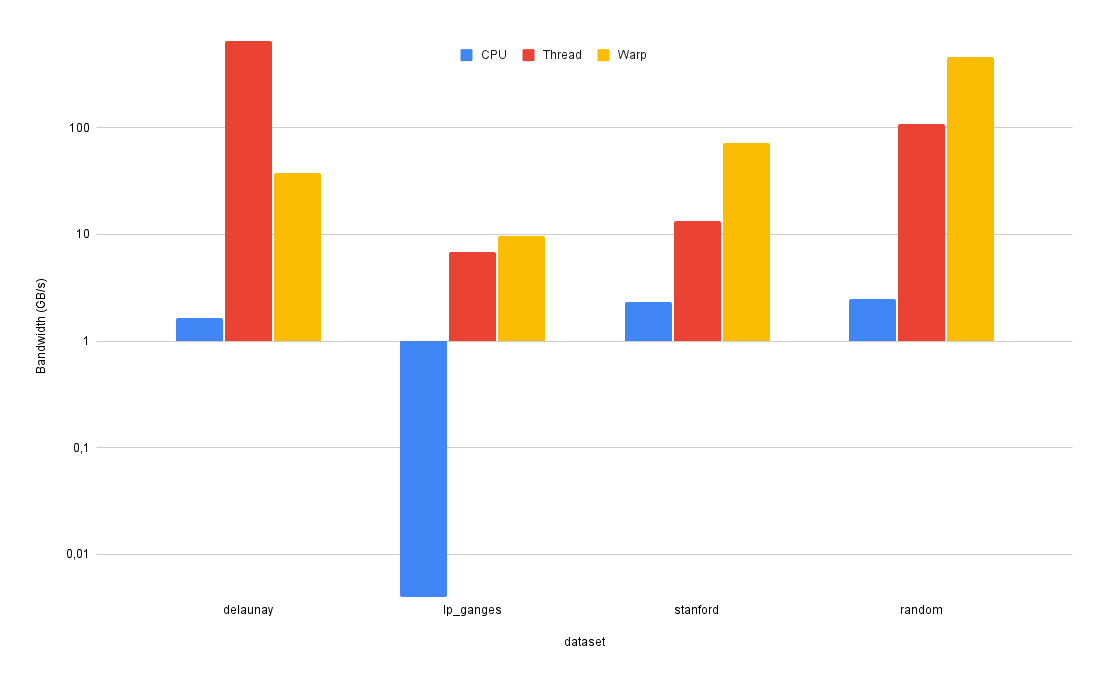
\includegraphics[width=0.95\linewidth]{images/chart.png}
    \caption{Bandwidths of the algorithms on the different datasets}
    \label{fig:chart}
\end{figure}

Lastly, \textit{cachegrind} has been used to measure the amount of cache misses. On the random matrix the naive CPU implementation gets 0.6\% D1 miss rate and 0.1\% LL miss rate. These results confirm that simply using the CSR format ensures a good usage of the cache.

\section{Conclusions}
% [max 200 words]\\
% Summarize findings and future work \dots
The use of the CSR format to store the matrix in memory has proven to be a useful tool to optimize the SpMV operation. The ordering of the elements based on their position in the matrix allows for a sequential access that is predictable and that can take good advantage of the cache.

Parallelization was shown to be orders of magnitude faster than the sequential operation on all datasets, with varying results on the kind of parallelization that yield the better performance.

Lastly, the attempt to find a better memory access pattern was unsuccessful. The trade-offs made when using the chunk based approach were likely too disadvantageous to bring any improvement.

\subsection{Future works}
As discussed earlier, there is a trend of improvement when moving from the first GPU implementation to the second one, with the exception of the results taken on the Delaunay Graph dataset. Further testing on different kinds of matrices could help determine whether this was a one-of occurrence or a common one.

Another improvement would be to use more threads for each row of the matrix being processed. This can however complicate the synchronization between threads if the implementation is not well thought out

Lastly, the use of global memory to store the buffer with the partial results of operations is an obvious slowdown. Future implementations would use shared memory and a better reduction algorithm to add together the partial sums.

\bibliographystyle{IEEEtran}
\bibliography{references}
\end{document}

